\documentclass[14pt]{extarticle}

\usepackage[T1]{fontenc}
\usepackage[utf8]{inputenc}
\usepackage[spanish]{babel}
\usepackage{geometry}
\usepackage{graphicx}
\usepackage{xcolor}
\usepackage{array}
\usepackage{booktabs}
\usepackage{colortbl}
\usepackage{hyperref}
\usepackage{lmodern}

\geometry{
  paperwidth=59.4cm,
  paperheight=84.1cm,
  margin=1.0cm
}

\graphicspath{{../latex/figures/}}
\pagestyle{empty}
\setlength{\parindent}{0pt}
\setlength{\parskip}{0.24em}
\renewcommand{\familydefault}{\sfdefault}
\renewcommand{\arraystretch}{1.12}

\definecolor{navy}{HTML}{103654}
\definecolor{teal}{HTML}{1C7C7D}
\definecolor{gold}{HTML}{D79B2E}
\definecolor{soft}{HTML}{EEF4F7}
\definecolor{softgold}{HTML}{FDF6E5}
\definecolor{textgray}{HTML}{1F252B}
\definecolor{linegray}{HTML}{D8E1E8}

\hypersetup{
  colorlinks=true,
  linkcolor=navy,
  urlcolor=teal
}

\newcommand{\Ang}{\AA}

\newcommand{\paneltitle}[1]{%
  \par\medskip
  \noindent
  \begin{tabular}{@{}p{0.45cm}@{\hspace{0.35em}}p{\dimexpr\linewidth-0.8cm\relax}@{}}
    \cellcolor{gold}\rule{0pt}{0.82cm} &
    \cellcolor{navy}\color{white}\bfseries\Large\rule{0pt}{0.82cm}\hspace{0.35em}#1
  \end{tabular}
  \par\smallskip
}

\newcommand{\panelend}{%
  \par\smallskip
  {\color{linegray}\rule{\linewidth}{0.8pt}}
  \par\medskip
}

\newcommand{\metric}[3]{%
  \fcolorbox{navy}{white}{%
    \begin{minipage}[c][2.55cm][c]{0.235\textwidth}
      \centering
      {\fontsize{23}{25}\selectfont\bfseries\color{navy} #1\par}
      \vspace{0.08em}
      {\small\bfseries\color{teal} #2\par}
      \vspace{0.06em}
      {\small\color{textgray} #3\par}
    \end{minipage}
  }%
}

\newcommand{\callout}[1]{%
  \par\smallskip
  \noindent\setlength{\fboxrule}{1.1pt}\setlength{\fboxsep}{0.28cm}%
  \fcolorbox{gold}{softgold}{%
    \begin{minipage}{\dimexpr\linewidth-2\fboxsep-2\fboxrule\relax}
      \color{textgray}\small #1
    \end{minipage}
  }%
  \par\smallskip
}

\newcommand{\readingbox}[1]{%
  \par\smallskip
  \noindent\setlength{\fboxrule}{0.8pt}\setlength{\fboxsep}{0.20cm}%
  \fcolorbox{teal}{soft}{%
    \begin{minipage}{\dimexpr\linewidth-2\fboxsep-2\fboxrule\relax}
      \color{textgray}\small #1
    \end{minipage}
  }%
  \par\smallskip
}

\newcommand{\resulttile}[2]{%
  \fcolorbox{linegray}{white}{%
    \begin{minipage}[c][2.0cm][c]{0.47\linewidth}
      \centering
      {\Large\bfseries\color{navy} #1\par}
      {\small\color{textgray} #2\par}
    \end{minipage}
  }%
}

\begin{document}

\begin{minipage}[c]{0.11\textwidth}
  
\includegraphics[width=\linewidth]{logo_itam.pdf}
\end{minipage}
\hfill
\begin{minipage}[c]{0.68\textwidth}
  {\fontsize{27}{30}\selectfont\bfseries\color{navy}
  Precisión estructural real de AlphaFold2 tras corregir el mapeo PDB--UniProt\par}
  \vspace{0.12em}
  {\fontsize{16}{19}\selectfont\color{teal}
  Benchmark sistemático con SIFTS sobre 10,432 proteínas únicas \quad | \quad reducción de 35$\times$ en el error mediano aparente\par}
  \vspace{0.18em}
  {\normalsize \textbf{José Antonio Tapia Godínez} \quad | \quad Maestría en Ciencia de Datos, ITAM \quad | \quad jose.tapia@itam.mx\par}
  {\small Asesor: Dr.\ Edgar Francisco Román Rangel \quad | \quad Concurso de Posters de Titulación 2026\par}
\end{minipage}
\hfill
\begin{minipage}[c]{0.17\textwidth}
  \fcolorbox{navy}{navy}{%
    \begin{minipage}[c][2.45cm][c]{\dimexpr\linewidth-2\fboxsep\relax}
      \centering
      {\color{white}\fontsize{28}{30}\selectfont\bfseries Alpha\textcolor{gold}{Fold}2\par}
      \vspace{0.08em}
      {\color{white}\small Benchmark estructural · SIFTS\par}
    \end{minipage}
  }
\end{minipage}

\vspace{0.18cm}

\begin{center}
  
\includegraphics[width=0.55\linewidth,keepaspectratio]{protein_banner_faded.png}
\end{center}

{\footnotesize\color{textgray}\hfill Estructura proteica predicha por AlphaFold2 · \href{https://alphafold.ebi.ac.uk}{AlphaFold DB}}

\vspace{0.18cm}

\noindent
\metric{10,432}{proteínas únicas}{procesadas con SIFTS}
\hfill
\metric{1.26 \Ang}{RMSD mediano}{dataset diversificado}
\hfill
\metric{65.3\%}{predicciones $<2$ \Ang}{nivel útil para bioinformática}
\hfill
\metric{35$\times$}{reducción de error}{al usar mapeo SIFTS}

\vspace{0.20cm}

\callout{%
{\bfseries\color{navy}Hallazgo clave.}
Sin mapeo SIFTS, el benchmark exagera el error de AlphaFold2. Al corregir la correspondencia PDB--UniProt, el RMSD mediano cae de \textbf{22.54 \Ang} a \textbf{0.64 \Ang} en el subset validado, con un desempeño global de \textbf{1.26 \Ang}.%
}

\vspace{0.12cm}

\begin{minipage}[t]{0.485\textwidth}
\small

\paneltitle{Problema, datos y método}
\textbf{Problema.} Comparar PDB y AlphaFold2 por número de residuo, sin corregir cadena ni numeración, infla artificialmente el error estructural.

\textbf{Objetivo.} Cuantificar la precisión estructural real de AlphaFold2 con un pipeline reproducible basado en SIFTS y alineamiento Kabsch.

\textbf{Diseño del estudio.}
\begin{itemize}
  \item RCSB PDB + AlphaFold DB + SIFTS como fuentes principales.
  \item Un PDB representativo por identificador UniProt.
  \item 13,000 pares candidatos $\rightarrow$ 11,384 descargados $\rightarrow$ \textbf{10,432 procesados} con éxito.
  \item Subset validado de \textbf{5,115 pares} con inicio de mapeo explícito.
\end{itemize}

\textbf{Variables principales.}
\begin{itemize}
  \item Respuesta: RMSD de C$\alpha$ tras alineamiento Kabsch.
  \item Estructurales y químicas: longitud proteica, residuos mapeados, aminoácido y tipo de átomo.
\end{itemize}

\textbf{Justificación metodológica.} SIFTS resuelve los dos errores más comunes en benchmarks PDB--AF2: desfase de numeración y selección incorrecta de cadena. Kabsch es la solución rígida óptima para superposición.
\panelend

\paneltitle{Pipeline Analítico}
\begin{center}
  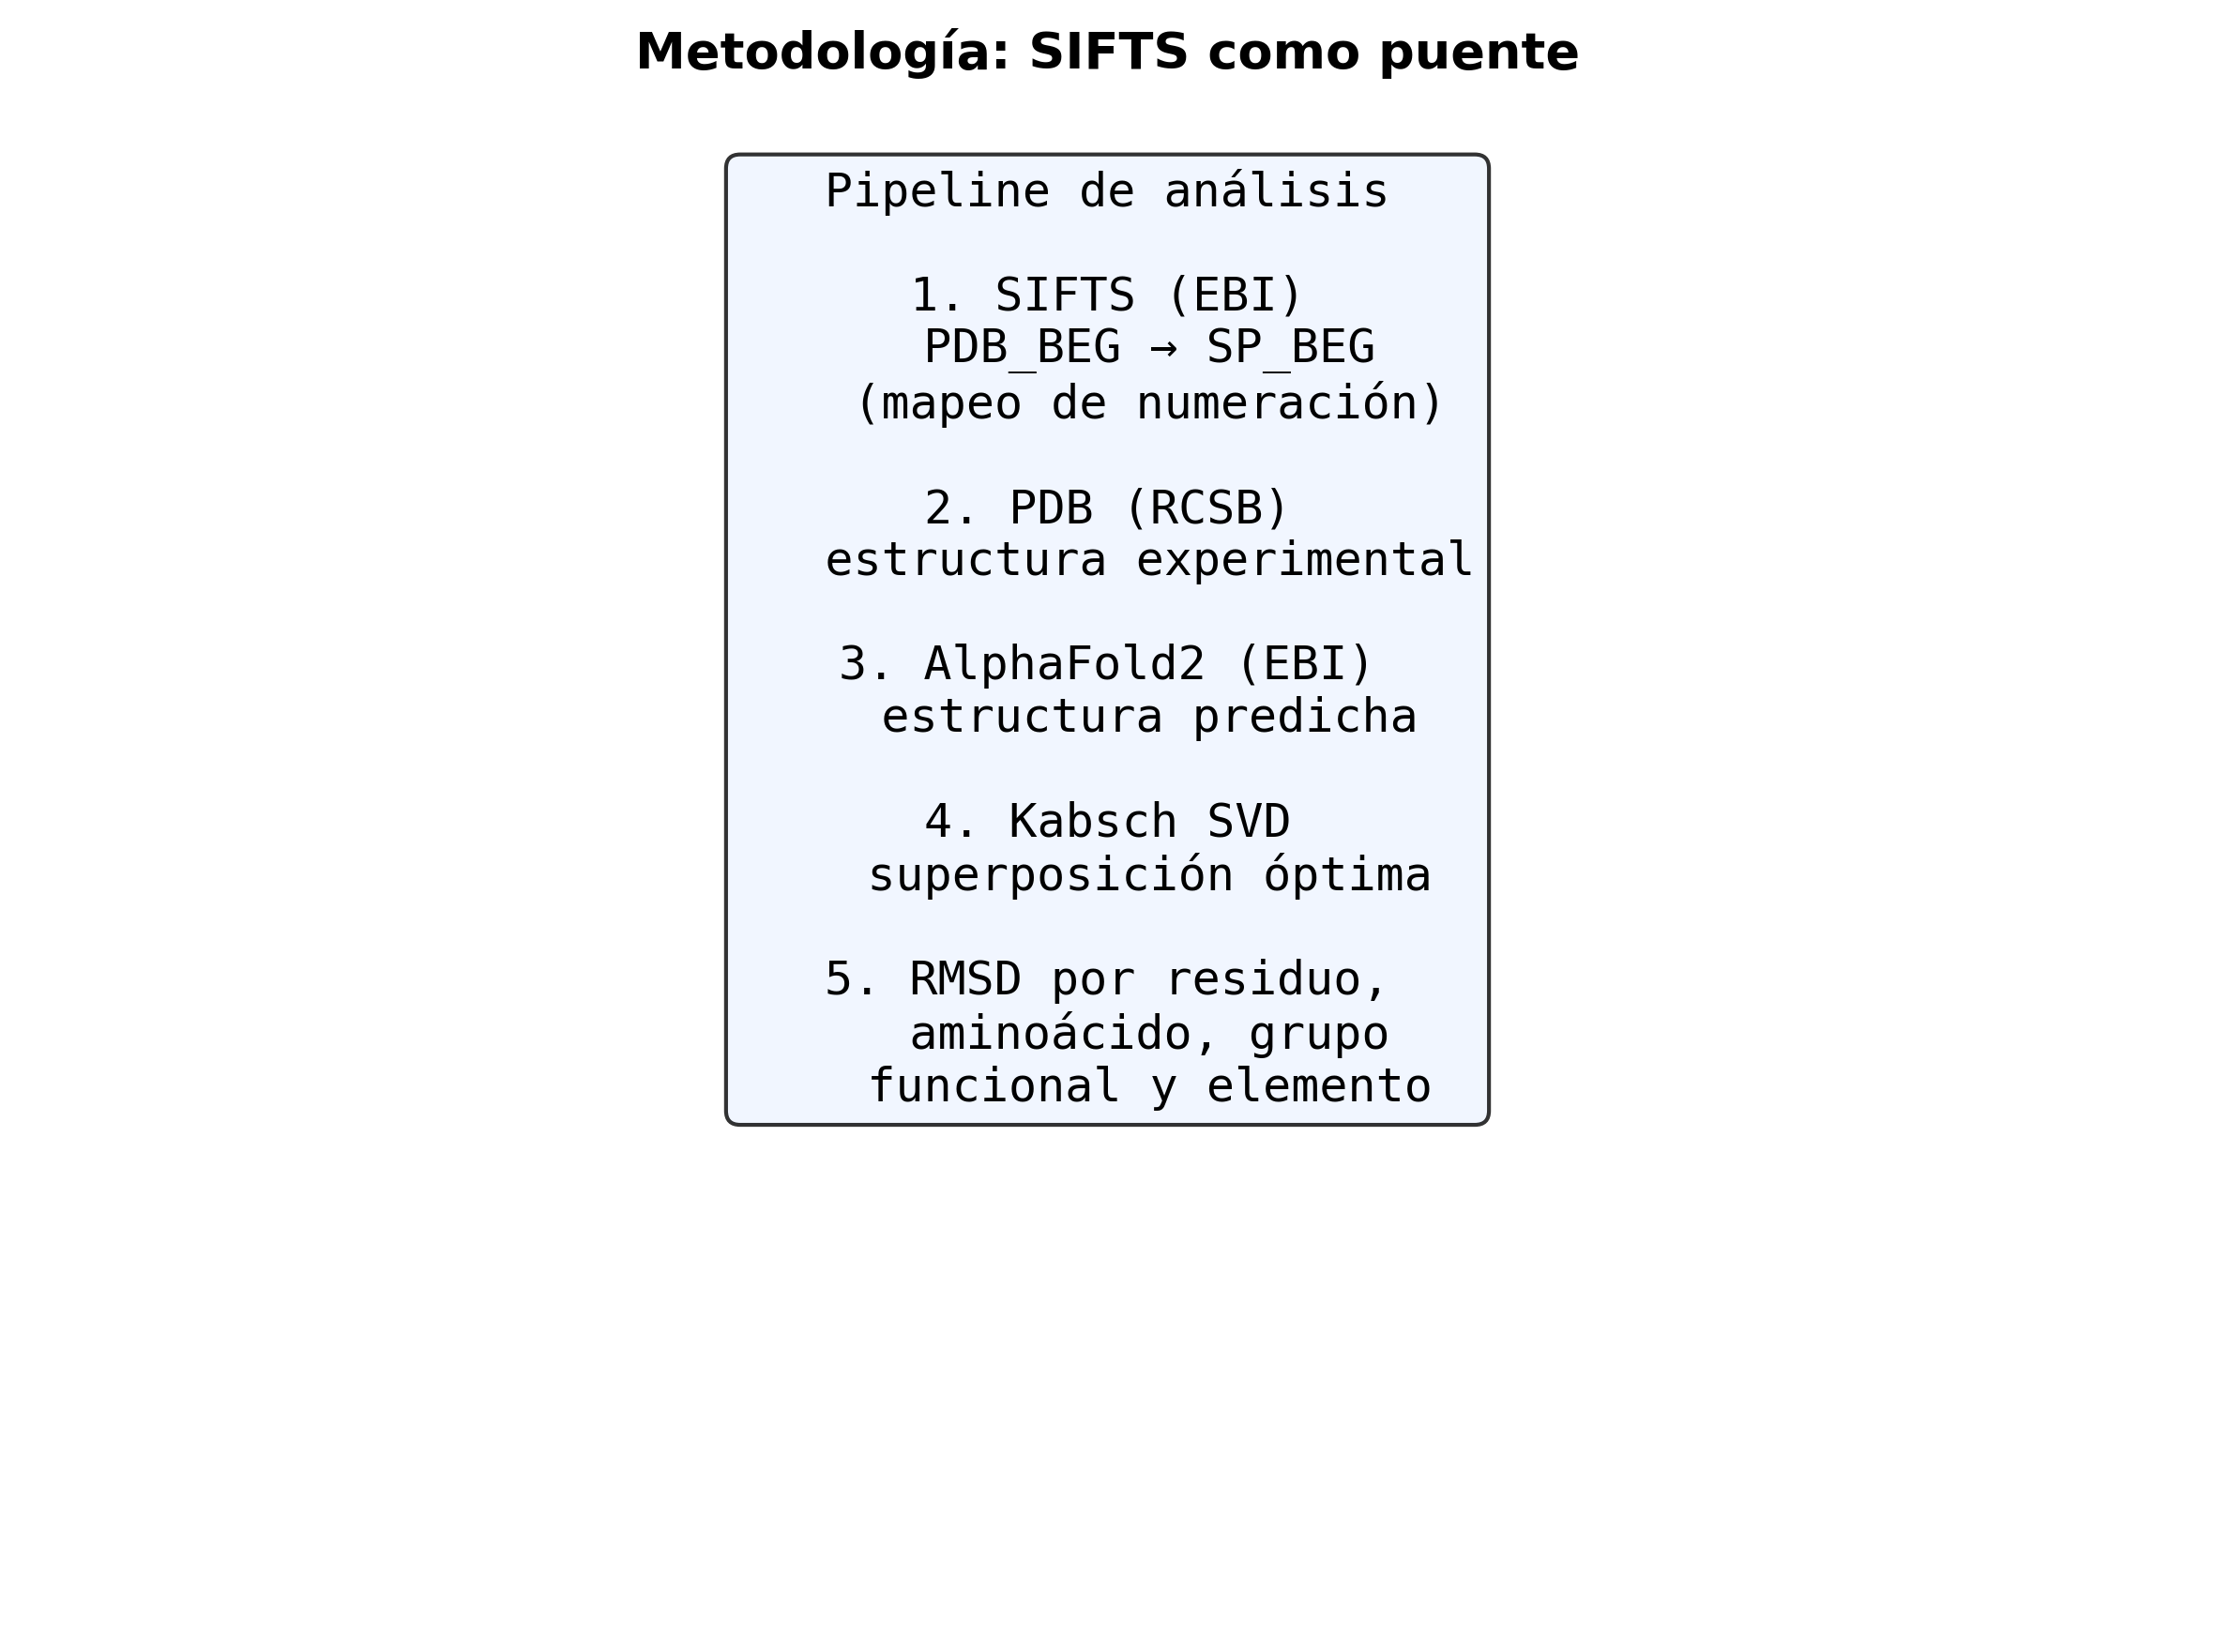
\includegraphics[width=0.92\linewidth]{fig_00a_pipeline.png}
\end{center}

\textbf{Flujo de trabajo.} Descarga $\rightarrow$ mapeo SIFTS $\rightarrow$ extracción de residuos comunes $\rightarrow$ superposición Kabsch $\rightarrow$ cálculo de RMSD $\rightarrow$ análisis estructural.

\textbf{Implementación.} Python 3, Biopython, NumPy, Pandas y Matplotlib/Seaborn.
\panelend

\paneltitle{El Cambio que Introduce SIFTS}
\begin{center}
  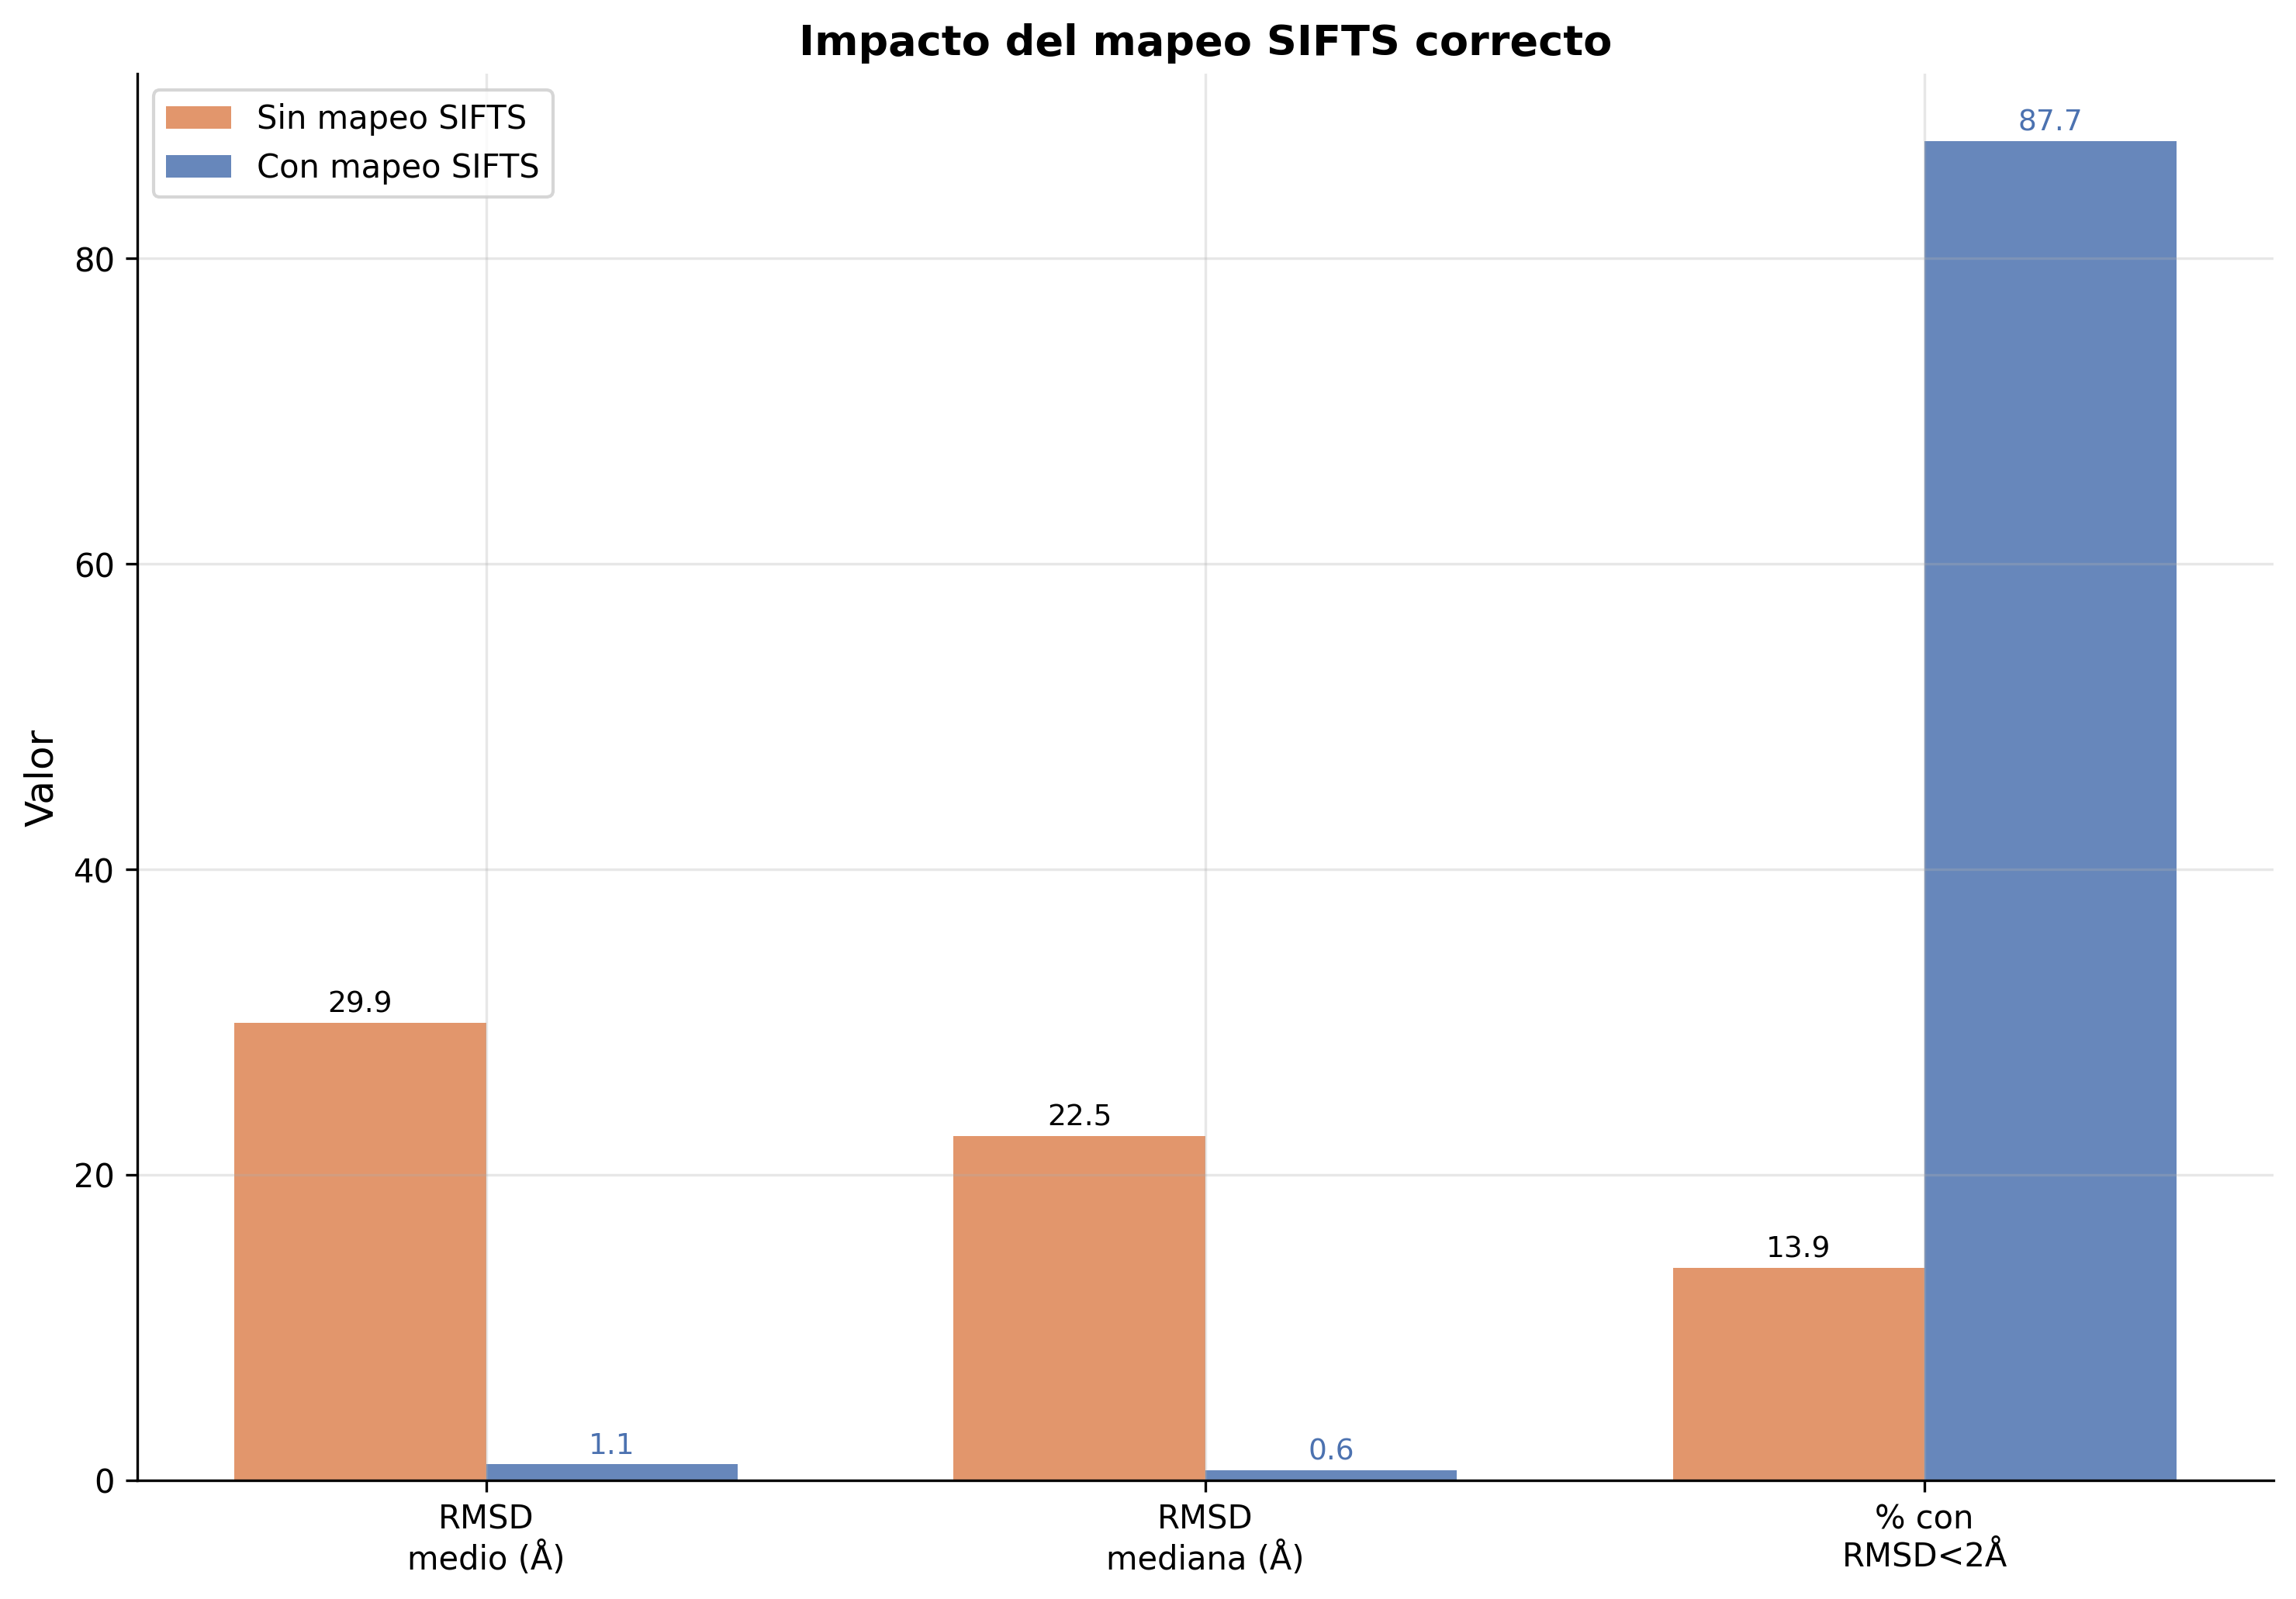
\includegraphics[width=0.94\linewidth]{fig_00b_sifts_comparison.png}
\end{center}

\resulttile{29.94 \Ang{} $\rightarrow$ 1.05 \Ang}{RMSD medio}
\hfill
\resulttile{22.54 \Ang{} $\rightarrow$ 0.64 \Ang}{RMSD mediano}

\vspace{0.16cm}

\resulttile{13.9\% $\rightarrow$ 87.7\%}{Predicciones con RMSD $<2$ \Ang}
\hfill
\resulttile{80.9\% $\rightarrow$ 0.4\%}{Predicciones con RMSD $>10$ \Ang}

\readingbox{%
\textbf{Lectura.} La mayor parte del error reportado por benchmarks ingenuos no provenía de AlphaFold2, sino de comparar residuos incorrectos. SIFTS cambia la interpretación completa del problema.%
}
\panelend

\end{minipage}
\hfill
\begin{minipage}[t]{0.485\textwidth}
\small

\paneltitle{Desempeño Global}
\begin{center}
  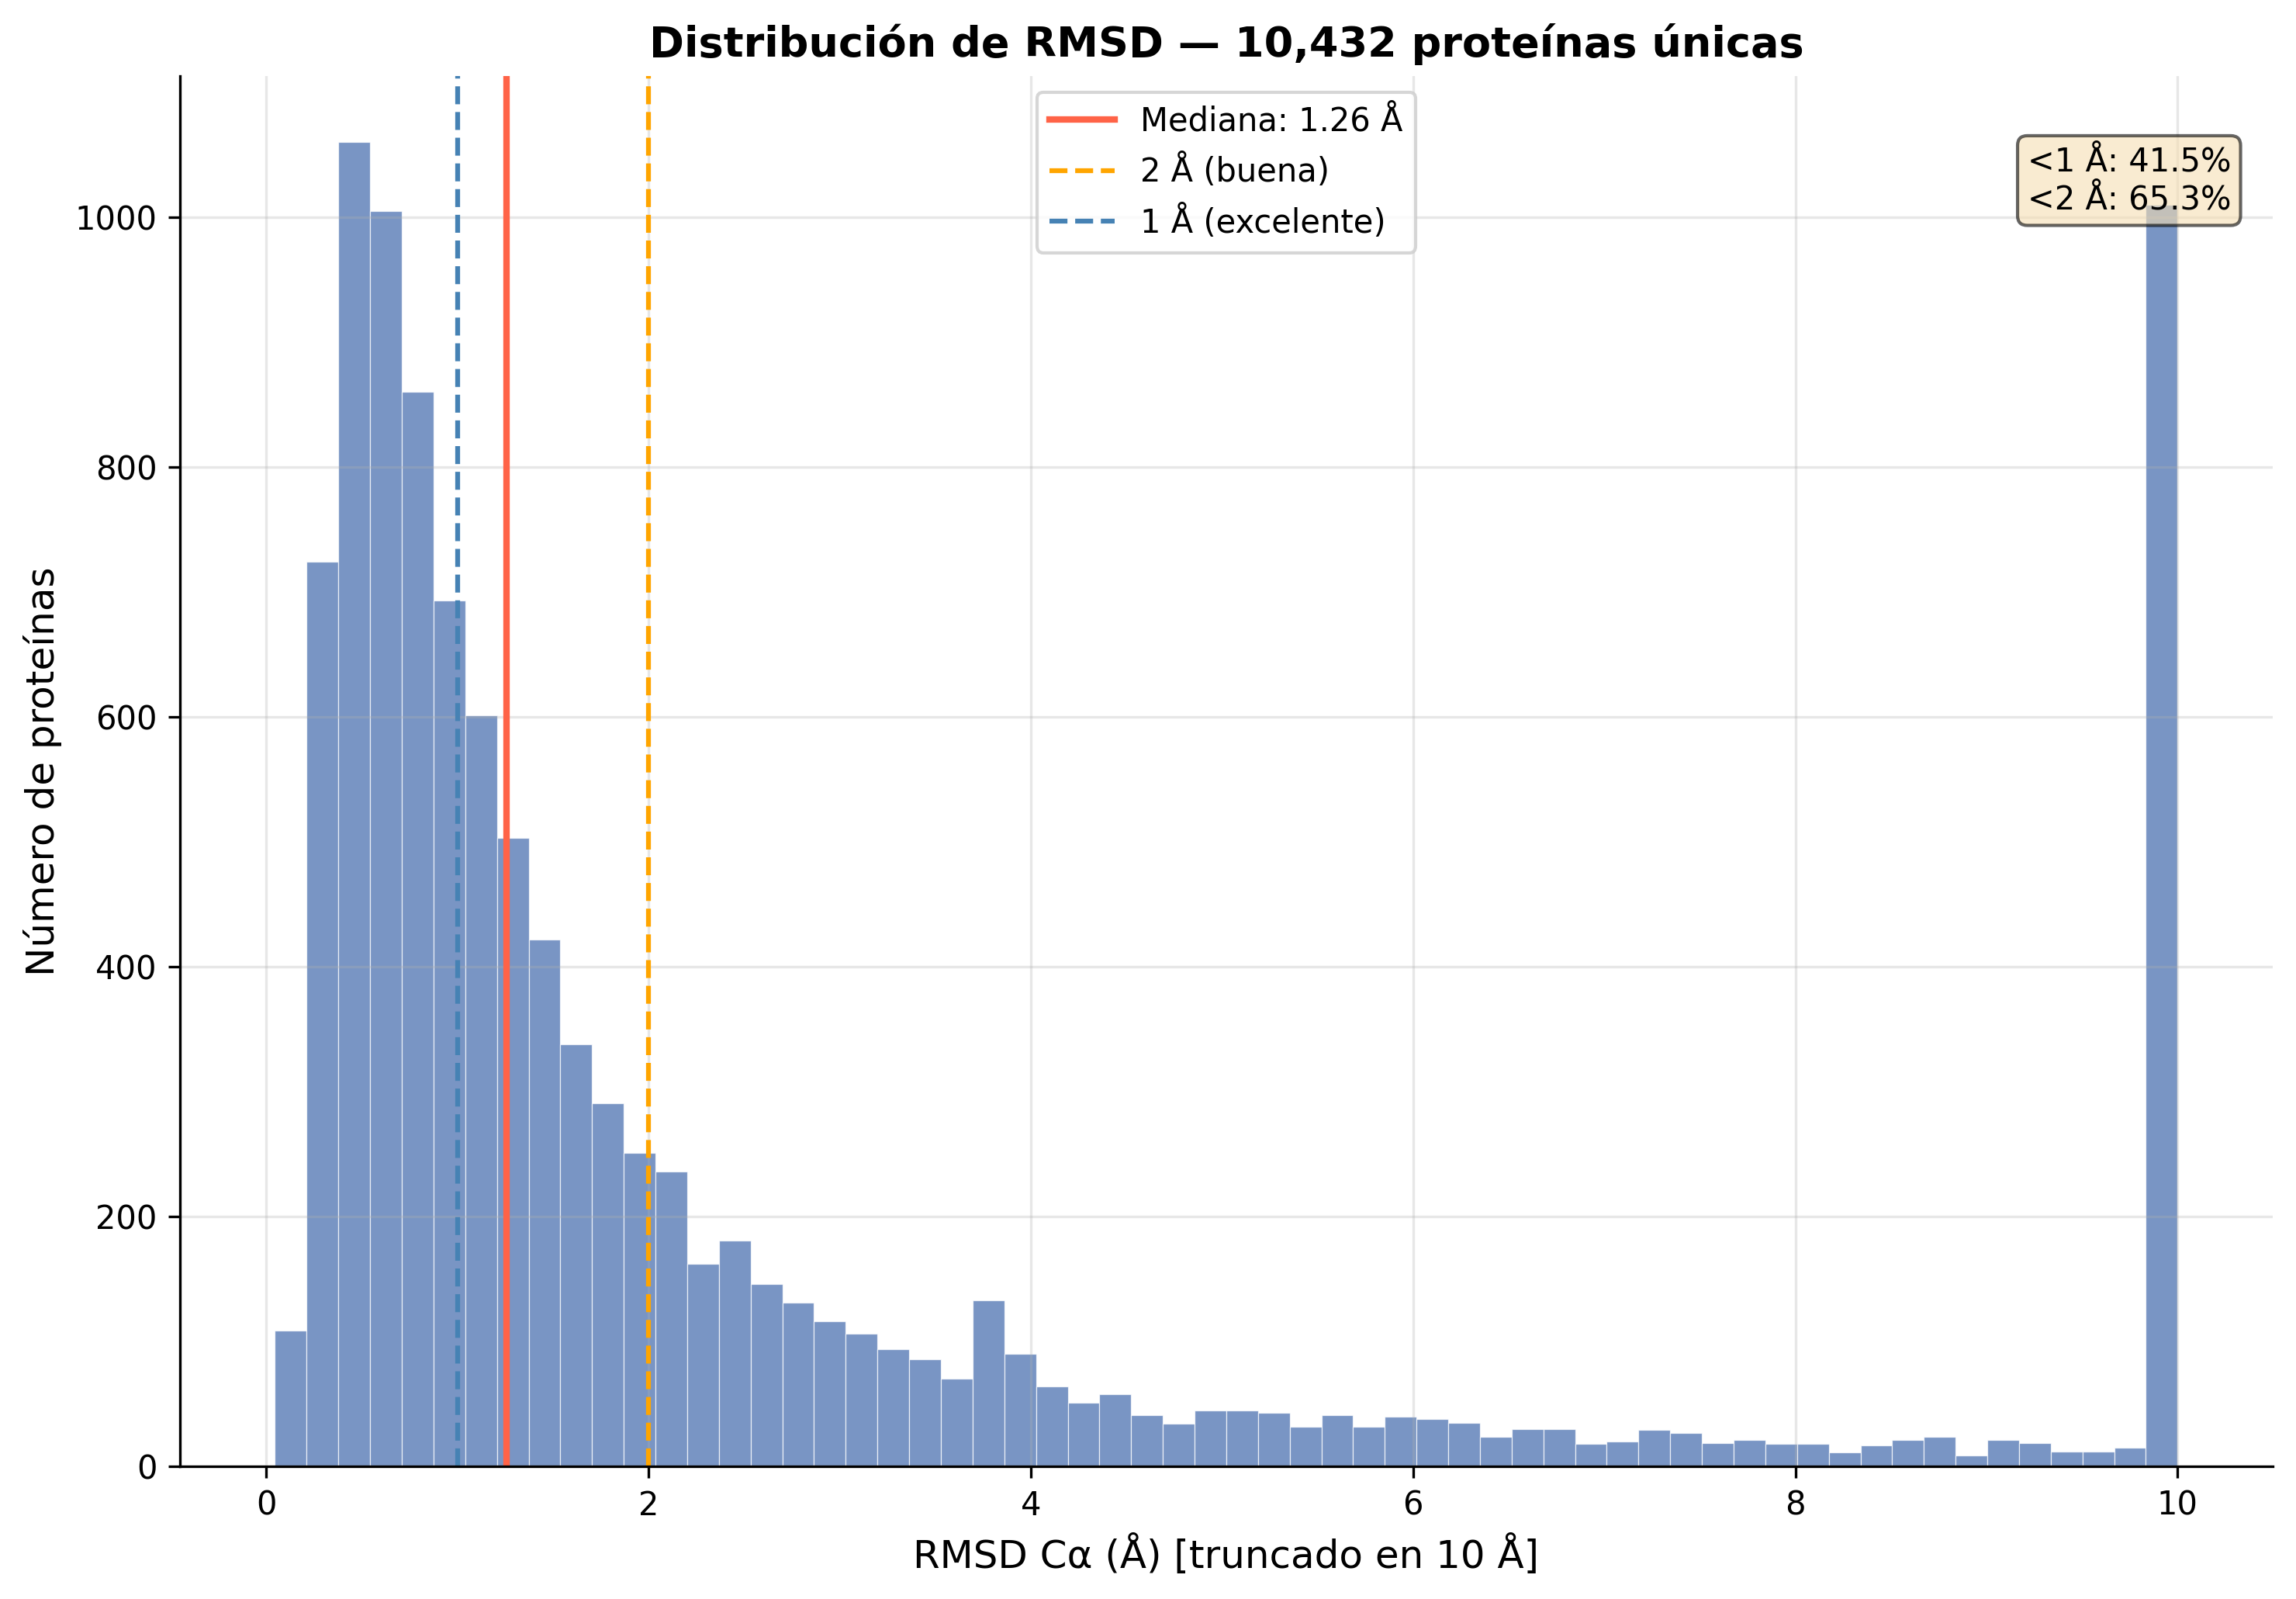
\includegraphics[width=0.94\linewidth]{fig_00c_rmsd_histogram.png}
\end{center}

\begin{itemize}
  \item \textbf{10,432 proteínas únicas} en el dataset diversificado final.
  \item \textbf{RMSD mediano: 1.26 \Ang}. RMSD medio: 3.56 \Ang.
  \item \textbf{41.5\%} con RMSD $<1$ \Ang{} y \textbf{65.3\%} con RMSD $<2$ \Ang.
  \item La distribución tiene cola derecha; la mediana describe mejor el comportamiento típico.
\end{itemize}

\readingbox{%
\textbf{Lectura.} Para una fracción amplia del proteoma, AlphaFold2 alcanza precisión estructural en el rango útil para bioinformática estructural y modelado molecular.%
}
\panelend

\paneltitle{Efecto del Tamaño Proteico}
\begin{center}
  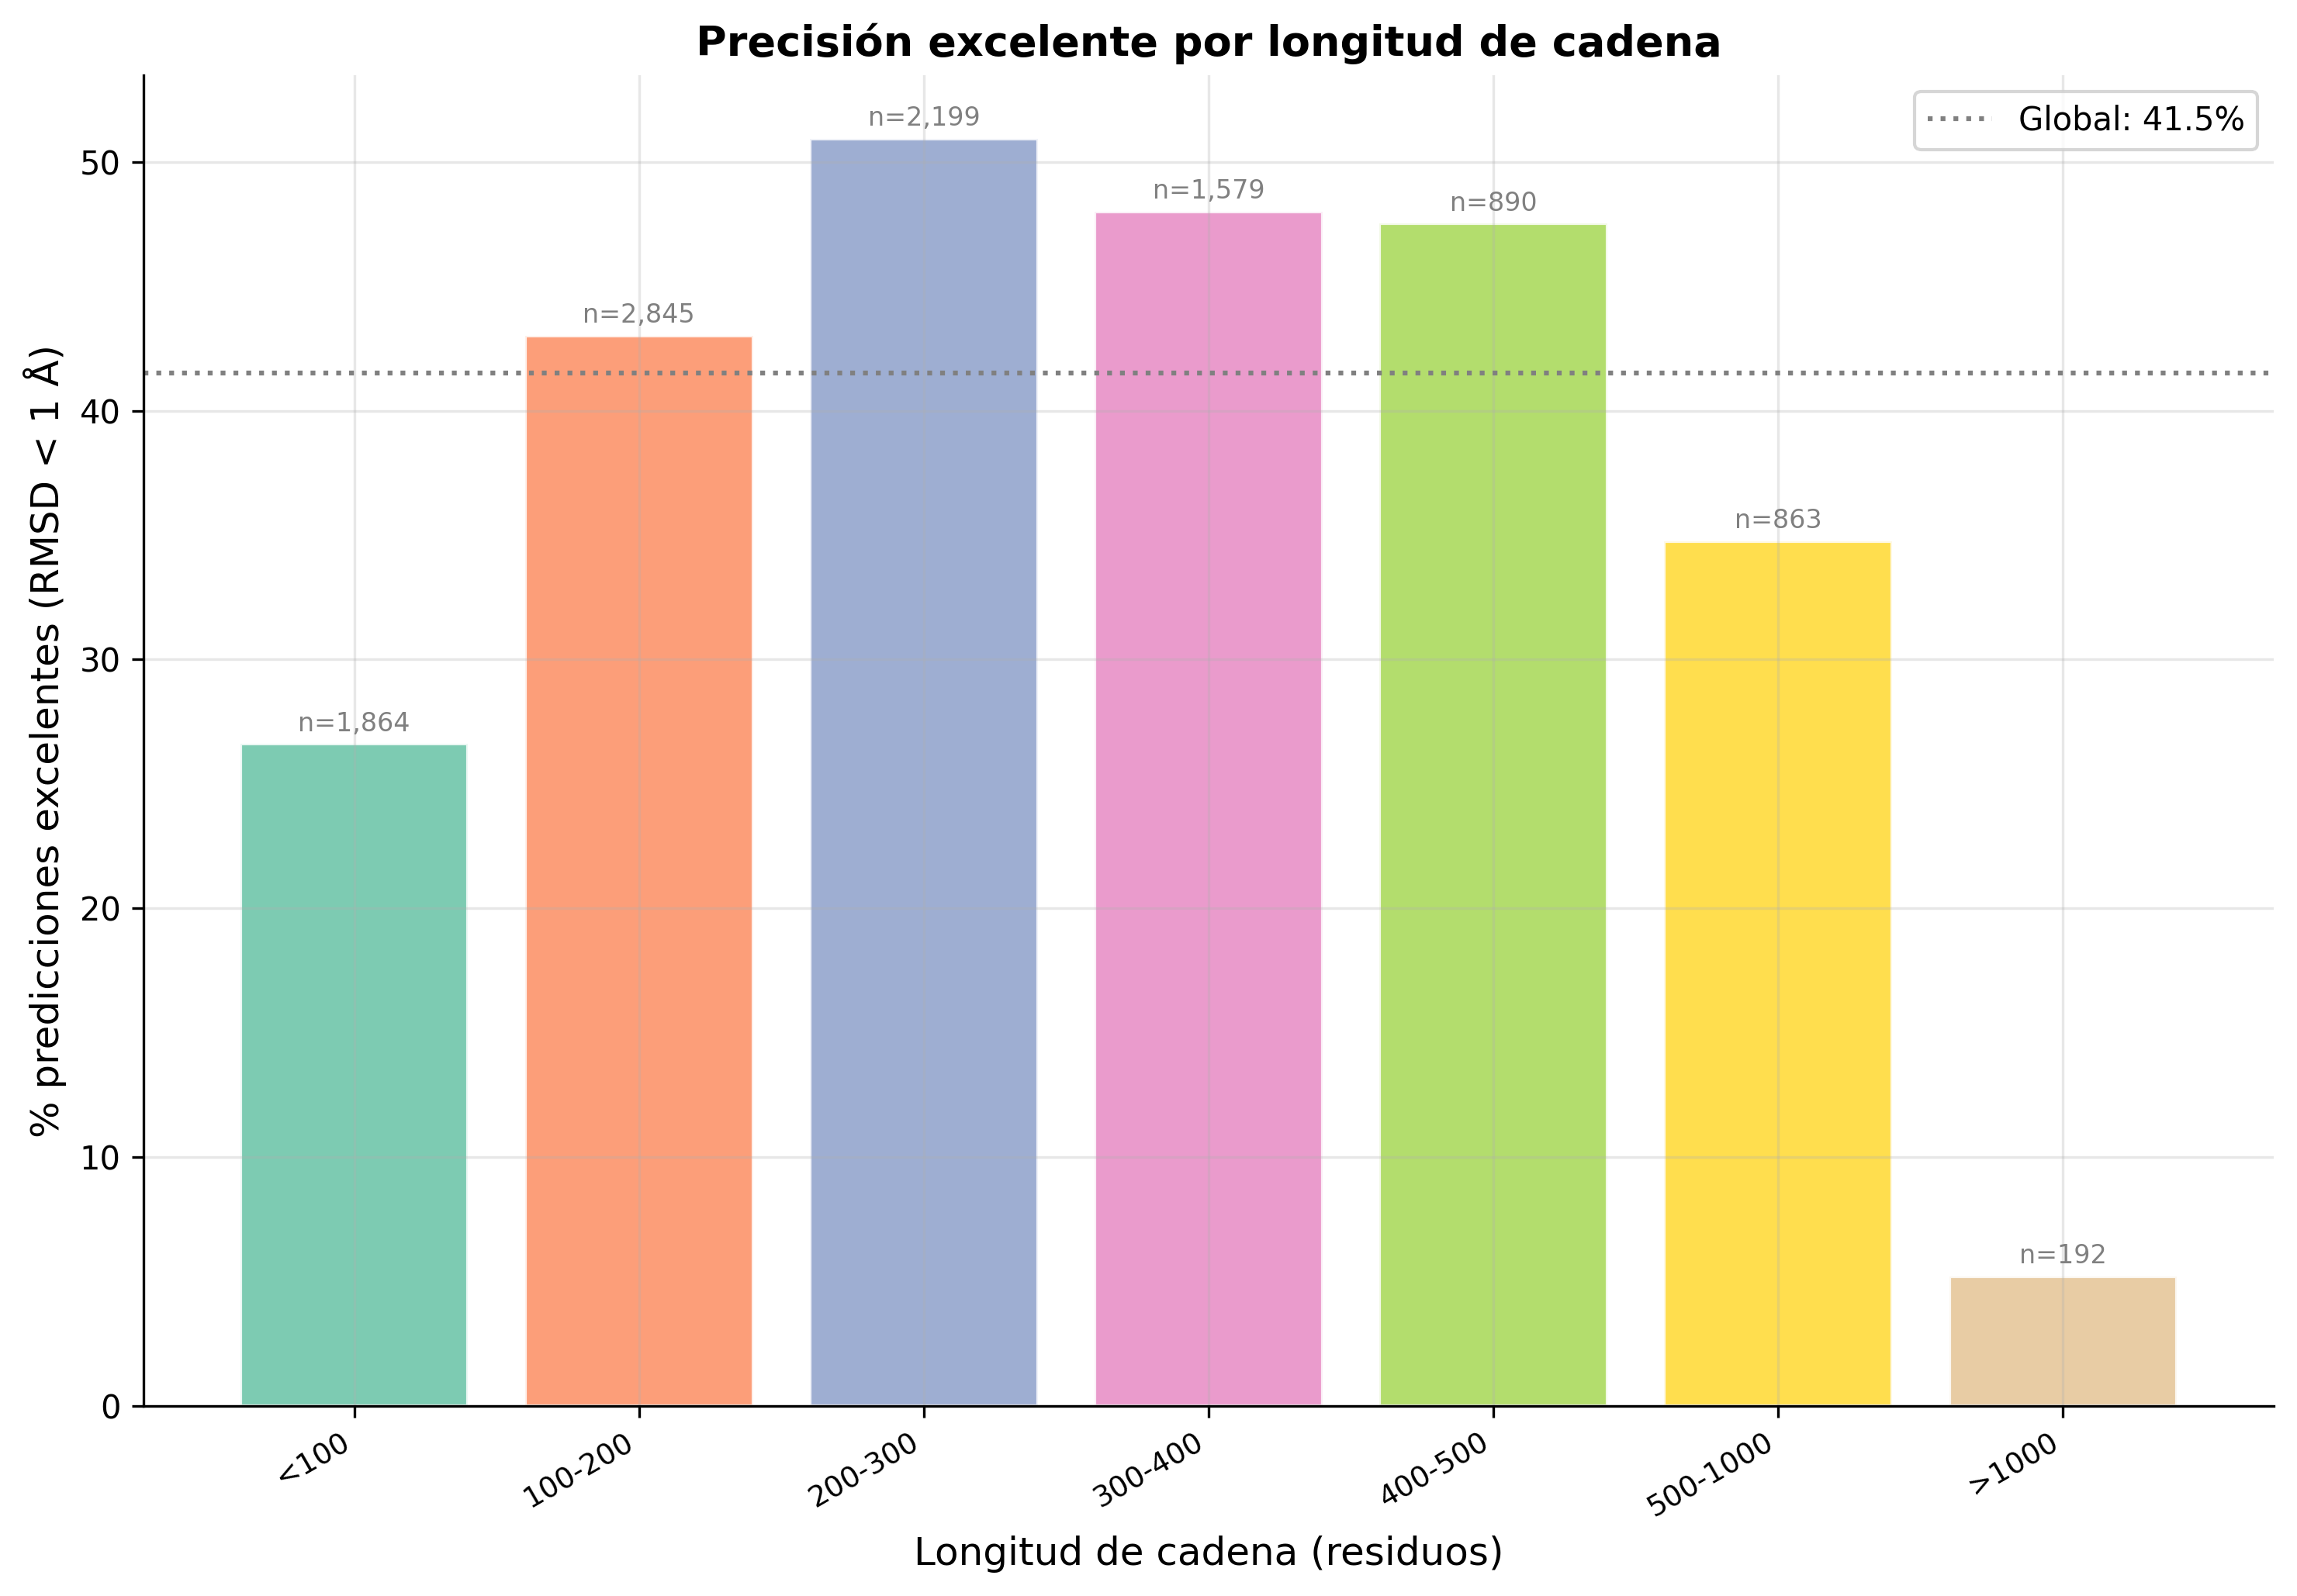
\includegraphics[width=0.94\linewidth]{fig_00d_excellence_by_length.png}
\end{center}

\begin{itemize}
  \item No aparece un \textit{sweet spot} universal y rígido de 250--300 residuos.
  \item Los rangos \textbf{200--300} y \textbf{300--400} mantienen métricas especialmente fuertes.
  \item El deterioro importante se concentra en proteínas muy grandes, por arriba de \textbf{1000 residuos}.
\end{itemize}

\textbf{Ejemplos cuantitativos.}
\begin{itemize}
  \item 200--300 residuos: mediana 0.98 \Ang{} y 51.1\% excelentes.
  \item 300--400 residuos: mediana 1.05 \Ang{} y 47.9\% excelentes.
  \item $>1000$ residuos: mediana 4.68 \Ang{} y 5.2\% excelentes.
\end{itemize}
\panelend

\paneltitle{Conclusiones e Impacto}
\begin{itemize}
  \item \textbf{AlphaFold2 alcanza alta precisión estructural} en el dataset analizado: RMSD mediano global de 1.26 \Ang.
  \item \textbf{SIFTS no es opcional}: es un requisito metodológico para comparar PDB y AlphaFold de forma válida.
  \item El supuesto \textit{sweet spot} 250--300 era sobre todo un artefacto del desfase de numeración.
  \item Los outliers se explican por conformaciones apo/holo, dominios móviles, desorden intrínseco o mapeos incompletos.
  \item El pipeline es \textbf{reproducible y transferible} a AlphaFold3 y otros predictores estructurales.
\end{itemize}

\textbf{Aplicaciones prácticas.}
\begin{itemize}
  \item \textit{Docking} molecular y \textit{virtual screening}
  \item Diseño racional, modelado por homología y anotación funcional
\end{itemize}
\panelend

\end{minipage}

\vfill

\noindent\fcolorbox{navy}{soft}{%
  \begin{minipage}{\dimexpr\textwidth-2\fboxsep-2\fboxrule\relax}
    {\small \textbf{\color{navy}Reproducibilidad.}
    Código y reporte: github.com/AntonioIQ/alphafold-project \quad | \quad
    \textbf{\color{navy}Compilación:} make poster \quad | \quad
    \textbf{\color{navy}Datos:} RCSB PDB, AlphaFold DB y SIFTS \quad | \quad
    \textbf{\color{navy}Citas clave:} Jumper et al.\ (2021), Varadi et al.\ (2022), Velankar et al.\ (2013).}
  \end{minipage}
}

\end{document}
